\documentclass[conference]{IEEEtran}
\usepackage[utf8]{inputenc}
\usepackage[T1]{fontenc}
\usepackage[turkish]{babel}
\usepackage{cite}
\usepackage{amsmath,amssymb,amsfonts}
\usepackage{algorithmic}
\usepackage{algorithm}
\usepackage{graphicx}
\usepackage{textcomp}
\usepackage{xcolor}
\usepackage{hyperref}
\usepackage{booktabs}
\usepackage{multirow}
\usepackage{float}

\hypersetup{
  colorlinks=true,
  linkcolor=blue,
  citecolor=blue,
  urlcolor=blue
}

% Fix IEEEtran.bst + babel-turkish compatibility
\makeatletter
\providecommand{\BIBentryALTinterwordspacing}{\spaceskip=0pt plus 0.3em minus 0.1em\relax}
\providecommand{\BIBentrySTDinterwordspacing}{\spaceskip=0pt\relax}
\makeatother

\begin{document}
\shorthandoff{=}

\title{Word Crush: Flutter Tabanlı Türkçe Kelime Bulma Mobil Oyunu}

\author{
\IEEEauthorblockN{Enes Demir}
\IEEEauthorblockA{
Bilgisayar Mühendisliği Bölümü \\
Kocaeli Üniversitesi \\
Kocaeli, Türkiye \\
230202066}
\and
\IEEEauthorblockN{Mert Şengül}
\IEEEauthorblockA{
Bilgisayar Mühendisliği Bölümü \\
Kocaeli Üniversitesi \\
Kocaeli, Türkiye \\
230202095}
}

\maketitle

\begin{abstract}
Bu çalışmada, mobil platformlar için geliştirilen ``Word Crush'' adlı Türkçe kelime bulma oyunu sunulmaktadır. Uygulama, iki boyutlu kare bir harf tahtası üzerinde oyuncunun komşu harfleri sürükleyerek anlamlı Türkçe kelimeler oluşturmasına dayanan tek oyunculu bir kelime oyunudur. Sistem; Türkçe harf frekanslarına dayalı ağırlıklı harf üretim algoritması, Trie veri yapısı tabanlı tahta analiz mekanizması, yerçekimi ve yeniden doldurma mekanikleri, SQLite ile yerel veri kalıcılığı, oyun içi market ve joker ekonomisi, aktif oturumun yerel olarak sürdürülmesi, combo puanlama ve kelime uzunluğuna bağlı özel güç üretimi gibi bileşenleri içerir. Başlangıç tahtasının ve hamle sonrası oluşan tahtaların oynanabilir kalmasını sağlamak amacıyla DFS tabanlı tahta analiz algoritması ile Fisher-Yates karıştırma temelli çok aşamalı kurtarma stratejileri uygulanmıştır. Uygulama tamamen çevrimdışı çalışmakta olup herhangi bir sunucu bağımlılığı taşımamaktadır.
\end{abstract}

\begin{IEEEkeywords}
Mobil oyun geliştirme, Flutter, kelime oyunu, Trie veri yapısı, SQLite, ağırlıklı harf üretimi, oyun mekanikleri, DFS
\end{IEEEkeywords}

% ================================================================
\section{Giriş}
% ================================================================

Mobil oyunlar, günümüzde en yaygın yazılım uygulama alanlarından birini oluşturmakta ve geniş bir kullanıcı kitlesine ulaşmaktadır. Kelime tabanlı oyunlar, hem dilsel becerileri geliştirmesi hem de stratejik düşünmeyi teşvik etmesi nedeniyle eğitici ve eğlenceli bir kategori olarak öne çıkmaktadır \cite{cormen_algorithms}.

Bu proje kapsamında, Kocaeli Üniversitesi Yazılım Laboratuvarı-II dersi için ``Word Crush'' adlı bir Türkçe kelime bulma mobil oyunu geliştirilmiştir. Oyunun temel amacı, oyuncunun kare bir harf tahtası üzerindeki harfleri parmak sürükleme ile birbirine bağlayarak anlamlı Türkçe kelimeler oluşturmasıdır. Geçerli bulunan kelimeler oyun alanından kaldırıldıktan sonra yerçekimi simülasyonu ile üstteki harfler aşağı düşer ve boş kalan alanlara yeni harfler üretilir. Oyuncu, sınırlı hamle sayısı içerisinde en yüksek puanı elde etmeye çalışmaktadır.

Uygulama, cross-platform mobil çerçeve kullanılarak geliştirilmiş olup Android ve iOS platformlarını hedeflemektedir \cite{flutter_overview}, \cite{dart_language}. Sistem tamamen yerel veri ile çalışmakta, herhangi bir uzak sunucu bağımlılığı taşımamakta ve kelime doğrulama için uygulama içine paketlenmiş kapsamlı bir Türkçe kelime listesinden yararlanmaktadır \cite{turkish_word_list}.

Bu raporun geri kalanında sırasıyla sistem mimarisi ve metodoloji, oyun mekanikleri, kullanıcı arayüzü tasarımı, test ve değerlendirme sonuçları ile sonuç ve gelecek çalışma yönleri sunulmaktadır.

% ================================================================
\section{Sistem Mimarisi ve Metodoloji}
% ================================================================

\subsection{Genel Mimari Yapı}

Uygulama, özellik tabanlı (feature-first) bir mimari yaklaşımla tasarlanmıştır. Bu yaklaşımda kod tabanı üç temel katmana ayrılmıştır: kullanıcı arayüzü katmanı, çekirdek oyun mantığı katmanı ve veri erişim katmanı. Katmanlar arasındaki bağımlılık yalnızca yukarı yönlüdür; oyun mantığı modülleri kullanıcı arayüzünden tamamen bağımsız olarak çalışabilir ve test edilebilir durumdadır.

Çekirdek oyun mantığı katmanı; tahta üretimi, kelime doğrulama, puanlama hesabı, yerçekimi çözümlemesi ve tahta çözülebilirlik analizi gibi saf algoritmaları içerir. Bu algoritmalar herhangi bir yan etki üretmez; tüm durum değişiklikleri çağrıcı katman tarafından yönetilir. Veri erişim katmanı ise kalıcı depolama ile uygulama arasındaki sınırı tanımlar ve repository tabanlı bir yapı sunar.

Şekil~\ref{fig:architecture} uygulamanın genel mimari yapısını göstermektedir.

\begin{figure}[H]
  \centering
  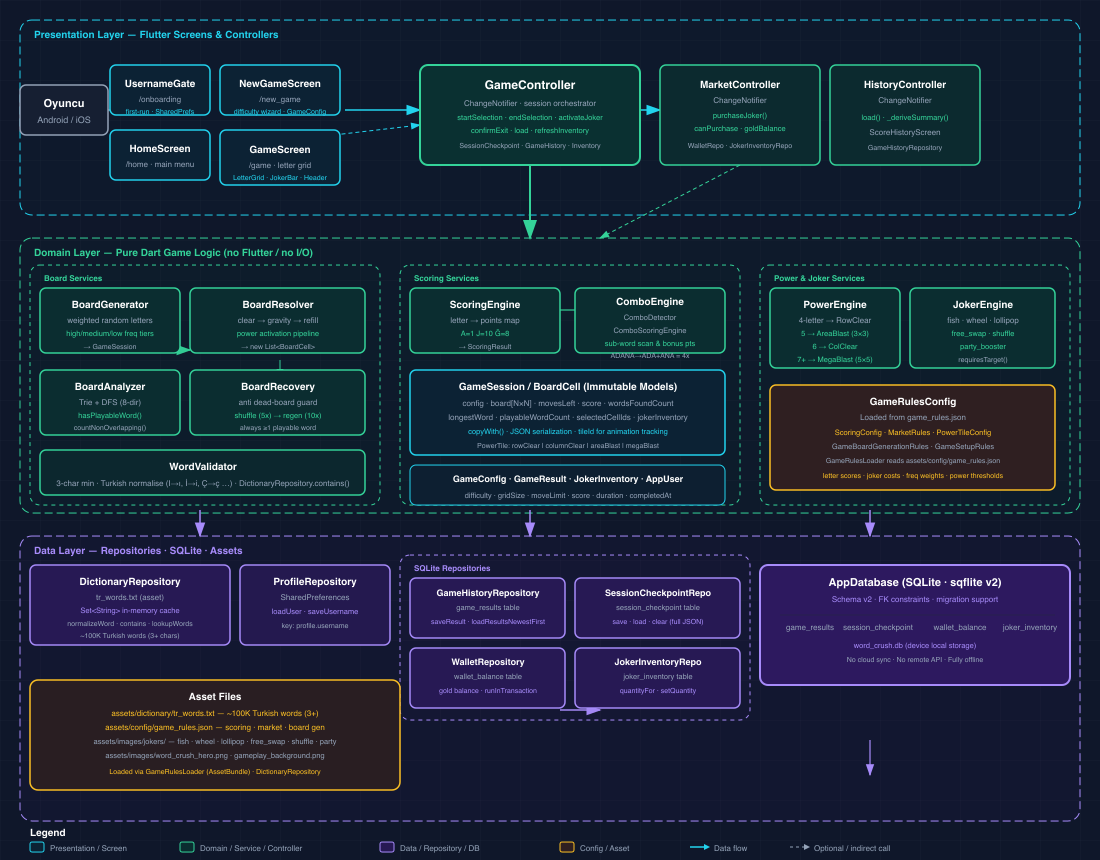
\includegraphics[width=0.95\linewidth]{architecture_diagram_only.png}
  \caption{Uygulamanın genel mimari yapısı}
  \label{fig:architecture}
\end{figure}

\subsection{Teknoloji Yığını}

Uygulama geliştirme sürecinde cross-platform mobil çerçeve olarak Flutter tercih edilmiştir \cite{flutter_overview}. Programlama dili olarak tip-güvenli yapısıyla Dart kullanılmıştır \cite{dart_language}. Kalıcı veri yönetiminde ilişkisel yerel veritabanı olarak SQLite \cite{sqflite_package}, hafif profil bilgileri için ise key-value tabanlı yerel depolama \cite{shared_preferences_package} seçilmiştir. Kullanıcı arayüzü bileşenleri Material Design 3 tasarım ilkeleri çerçevesinde oluşturulmuştur \cite{material_design}.

\subsection{Veri Yönetimi Stratejisi}

Kalıcı veri yönetimi iki farklı depolama mekanizmasına ayrılmıştır. Kullanıcı adı gibi tekil, basit verilerin saklanmasında key-value tabanlı hafif bir yerel depo kullanılmaktadır \cite{shared_preferences_package}. Oyun geçmişi, altın bakiyesi, joker envanteri ve aktif oturum verileri gibi yapısal ve ilişkisel verilerin yönetiminde ise SQLite tabanlı yerel bir ilişkisel veritabanı tercih edilmiştir \cite{sqflite_package}, \cite{sqlite_docs}.

Veritabanı şemasında dört temel tablo tanımlanmıştır: tamamlanan oyun sonuçlarını kaydeden sonuç tablosu, aktif oyun durumunu saklayan oturum kontrol noktası tablosu, oyuncunun altın bakiyesini yöneten cüzdan tablosu ve satın alınan joker miktarlarını tutan envanter tablosu. Şema sürümlemesi ve tablo oluşturma işlemleri merkezi bir veritabanı yönetim bileşeni tarafından kontrol edilmektedir.

% ================================================================
\section{Oyun Mekanikleri}
% ================================================================

\subsection{Oyun Akışı}

Oyun akışı dört ana aşamadan oluşmaktadır. İlk aşamada kullanıcı adı kaydı ve saklanması gerçekleştirilir. İkinci aşamada oyuncu ana ekrandan ``Yeni Oyun'' seçeneğini kullanarak önce grid boyutunu, ardından hamle sayısını seçer. Üçüncü aşamada seçilen parametrelere uygun bir harf tahtası oluşturularak aktif oyun başlar. Dördüncü aşamada oyun sona erdiğinde sonuç yerel veritabanına kaydedilir ve oyuncu ana ekrana yönlendirilir.

\subsection{Ağırlıklı Harf Üretim Algoritması}

Türkçe dilinde harflerin kullanım frekansları önemli ölçüde farklılık göstermektedir. Tamamen rastgele harf üretimi durumunda anlamlı kelime oluşturma olasılığı ciddi biçimde düşeceğinden, harfler Türkçe frekans dağılımına uygun ağırlıklı bir algoritma ile üretilmektedir \cite{turkce_frekans}.

Harf havuzu üç frekans kademesinden oluşmaktadır. Bu kademeler ve karşılık gelen harf kümeleri Tablo~\ref{tab:letter-frequency-groups} üzerinde özetlenmiştir. Harf üretim algoritması, toplam ağırlık havuzundan rastgele bir eşik değeri seçer ve ilgili kademe içerisinden harf üretimini gerçekleştirir.

\begin{table}[H]
\centering
\caption{Ağırlıklı harf üretiminde kullanılan frekans kademeleri}
\label{tab:letter-frequency-groups}
\begin{tabular}{lll}
\toprule
\textbf{Kademe} & \textbf{Ağırlık} & \textbf{Harfler} \\
\midrule
Yüksek frekans & 6 & A, E, İ, L, R, N \\
Orta frekans & 3 & K, M, T, S, Y, D \\
Düşük frekans & 1 & J, Ğ, F, V \\
\bottomrule
\end{tabular}
\end{table}

Bu ağırlıklı üretim yaklaşımı, tahtada Türkçe kelime oluşumunu kolaylaştıran doğal bir harf dağılımı sağlamaktadır.

\subsection{Kelime Seçimi ve Doğrulama Mekanizması}

Oyuncu, tahta üzerinde parmak sürükleme ile harf seçimi yapmaktadır. Seçim sırasında aşağıdaki kurallar uygulanır:

\begin{itemize}
  \item Her hücre bir kelime içerisinde yalnızca bir kez kullanılabilir.
  \item Seçim yalnızca 8 yönlü komşuluk ilişkisi (yatay, dikey ve çapraz) içerisinde ilerleyebilir.
  \item Seçilen kelime en az 3 harf uzunluğunda olmalıdır.
\end{itemize}

Oyuncu parmağını ekrandan kaldırdığında seçim tamamlanır ve kelime doğrulama mekanizması devreye girer. Bu mekanizma, oluşturulan kelimeyi Türkçe karakter normalizasyonu uygulayarak açık kaynaklı Türkçe kelime listesi \cite{turkish_word_list} üzerinde üyelik kontrolü ile doğrular. Doğrulama sonucuna göre kelime geçerli, sözlükte bulunmayan veya çok kısa olarak kategorize edilir.

Hem geçerli hem de geçersiz kelime denemeleri birer hamle harcar. Geçersiz bir deneme durumunda seçim iptal edilerek tahta eski haline döner; geçerli bir deneme ise puanlama ve harf temizleme akışını tetikler.

\subsection{Puanlama Sistemi}

Her harfe, Türkçe dilindeki kullanım sıklığı ve zorluğuna göre farklı puan değerleri atanmıştır. Uygulamada kullanılan tüm harf puanları, puan değerlerine göre gruplanmış biçimde Tablo~\ref{tab:letter-score-groups} üzerinde verilmiştir.

\begin{table}[H]
\centering
\caption{Harf puanlarının gruplu gösterimi}
\label{tab:letter-score-groups}
\begin{tabular}{ll}
\toprule
\textbf{Puan} & \textbf{Harfler} \\
\midrule
1 & A, E, İ, K, L, N, R, T \\
2 & I, M, O, S, U \\
3 & B, D, Ü, Y \\
4 & C, Ç, Ş, Z \\
5 & G, H, P \\
7 & F, Ö, V \\
8 & Ğ \\
10 & J \\
\bottomrule
\end{tabular}
\end{table}

Kelime puanı, kelimeyi oluşturan her harfin bireysel puanının toplamına eşittir. Örneğin ``DENİZ'' kelimesinin puanı D(3)+E(1)+N(1)+İ(1)+Z(4) = 10 olarak hesaplanmaktadır.

\subsection{Yerçekimi ve Yeniden Doldurma Mekaniği}

Geçerli bir kelime onaylandığında üç aşamalı bir çözümleme süreci başlatılır:

\begin{enumerate}
  \item \textbf{Temizleme}: Seçilen harfler oyun tahtasından kaldırılır.
  \item \textbf{Yerçekimi}: Her sütunda kalan harfler aşağı doğru kaydırılır; boş alanlar sütunun üst kısmında birikir.
  \item \textbf{Yeniden Doldurma}: Boş kalan pozisyonlar ağırlıklı harf üretim algoritması kullanılarak yeni harflerle doldurulur.
\end{enumerate}

Bu üç aşamalı çözümleme sürecinde temizleme ve yerçekimi adımları deterministik olarak işler; yeniden doldurma adımı ise ağırlıklı harf üretim algoritmasına dayalı rastlantısal seçim içerir. Süreç, mevcut tahta durumunu doğrudan değiştirmek yerine yeni bir tahta kopyası üretir.

\subsection{Tahta Çözülebilirlik Analiz Algoritması}

Oyuncuya gösterilen tahtanın her zaman en az bir geçerli kelime içermesi kritik bir gereksinimdir. Bu gereksinimi karşılamak üzere Trie veri yapısı \cite{trie_data_structure} ile DFS (Derinlik Öncelikli Arama) ve geri izleme (backtracking) \cite{dfs_backtracking} yöntemlerini birleştiren bir tahta analiz algoritması geliştirilmiştir.

Algoritma aşağıdaki adımları izler:

\begin{algorithm}[H]
\caption{Tahta Çözülebilirlik Analizi}
\begin{algorithmic}[1]
\STATE Sözlükten yalnızca $\geq$3 harfli kelimelerle bir Trie oluştur
\FOR{tahtadaki her hücre $h$}
  \STATE $h$'yi başlangıç noktası olarak seç
  \STATE Trie kökünden DFS+backtracking başlat
  \FOR{her 8-yönlü komşu $k$}
    \IF{$k$ daha önce ziyaret edilmediyse \AND Trie'da geçerli prefix varsa}
      \STATE Aramaya devam et
      \IF{terminal düğüme ulaşıldı \AND derinlik $\geq$ 3}
        \RETURN \textit{Geçerli kelime bulundu --- tahta oynanabilir}
      \ENDIF
    \ELSE
      \STATE Dalı buda (prefix pruning)
    \ENDIF
  \ENDFOR
  \STATE Geri izleme: $h$'yi ziyaret edilmemiş olarak işaretle
\ENDFOR
\RETURN \textit{Geçerli kelime bulunamadı --- tahta oynanamaz}
\end{algorithmic}
\end{algorithm}

Trie yapısı, arama sırasında geçersiz prefix'lerin erken budanmasını sağlayarak algoritmanın verimliliğini önemli ölçüde artırmaktadır. Algoritma, ilk geçerli kelimeyi bulduğu anda kısa devre ile sonlanır.

\subsection{Tahta Kurtarma Stratejisi}

Başlangıç tahtası ya da hamle sonrası oluşturulan tahta geçerli kelime içermediği durumlarda iki aşamalı bir kurtarma stratejisi devreye girmektedir:

\begin{enumerate}
  \item \textbf{Karıştırma aşaması}: Mevcut harfler, pozisyonları Fisher-Yates karıştırma algoritması \cite{fisher_yates_shuffle} ile yeniden düzenlenir. Bu işlem en fazla 5 deneme ile sınırlandırılmıştır.
  \item \textbf{Yeniden üretim aşaması}: Karıştırma başarılı olamazsa tamamen yeni bir tahta ağırlıklı harf üretim algoritması ile oluşturulur. Bu işlem en fazla 10 deneme ile sınırlandırılmıştır.
\end{enumerate}

Her iki aşamada da üretilen tahta, çözülebilirlik analiz algoritması ile doğrulanır. Bu strateji sayesinde oyuncuya kelime içermeyen bir tahta gösterilmemesi hedeflenmiş ve normal çalışma akışında bu durumun önüne geçilmiştir.

% ================================================================
\section{Kullanıcı Arayüzü Tasarımı}
% ================================================================

\subsection{Giriş ve Ana Ekran}

Uygulama ilk açıldığında oyuncudan kullanıcı adı girmesi istenir. Başarılı kayıt sonrasında bu isim yerel depolama alanında saklanır ve sonraki açılışlarda yeniden giriş gerektirmez. Ana ekranda üç temel navigasyon seçeneği sunulmaktadır: Yeni Oyun, Skor Tablosu ve Market. Kullanıcı adı, ana ekranın sol üst köşesinden değiştirilebilir olarak tasarlanmıştır.

\subsection{Oyun Kurulumu}

``Yeni Oyun'' seçildiğinde iki aşamalı bir kurulum akışı başlamaktadır. İlk aşamada oyuncuya üç grid boyutu sunulur: 6$\times$6 (Zor), 8$\times$8 (Orta) ve 10$\times$10 (Kolay). İkinci aşamada ise hamle sayısı paketleri gösterilir: 15, 20 ve 25. Seçim tamamlandığında oyun seçilen parametrelerle başlar.

\subsection{Oyun Ekranı}

Oyun ekranı, seçilen boyutta kare harf tahtasını, anlık puan göstergesini, kalan hamle sayacını, aktif kelime görüntüsünü ve mevcut tahtada ortak harf kullanmadan oluşturulabilecek kelime sayısını içerir. Bu değer, her hamle sonrasında tahta yeniden analiz edilerek güncellenmekte ve oyuncuya o anki gridin oynanabilirlik durumu hakkında anlık bilgi sağlamaktadır. Oyuncu parmak sürükleme ile komşuluk kuralına uygun harf seçimi yapmakta ve seçilen yol görsel olarak vurgulanmaktadır.

Kullanıcı deneyimini zenginleştirmek için çeşitli mikro-animasyonlar uygulanmıştır: geçersiz kelime denemelerinde tahta sarsma efekti, harf seçimi ve joker etkileri sırasında hareket animasyonları ile oyun ekranındaki skor alanında animasyonlu puan gösterimi. Şekil~\ref{fig:game_screen} oyun ekranının örnek görünümünü sunmaktadır.

\begin{figure}[H]
  \centering
  \setlength{\fboxsep}{0pt}\fbox{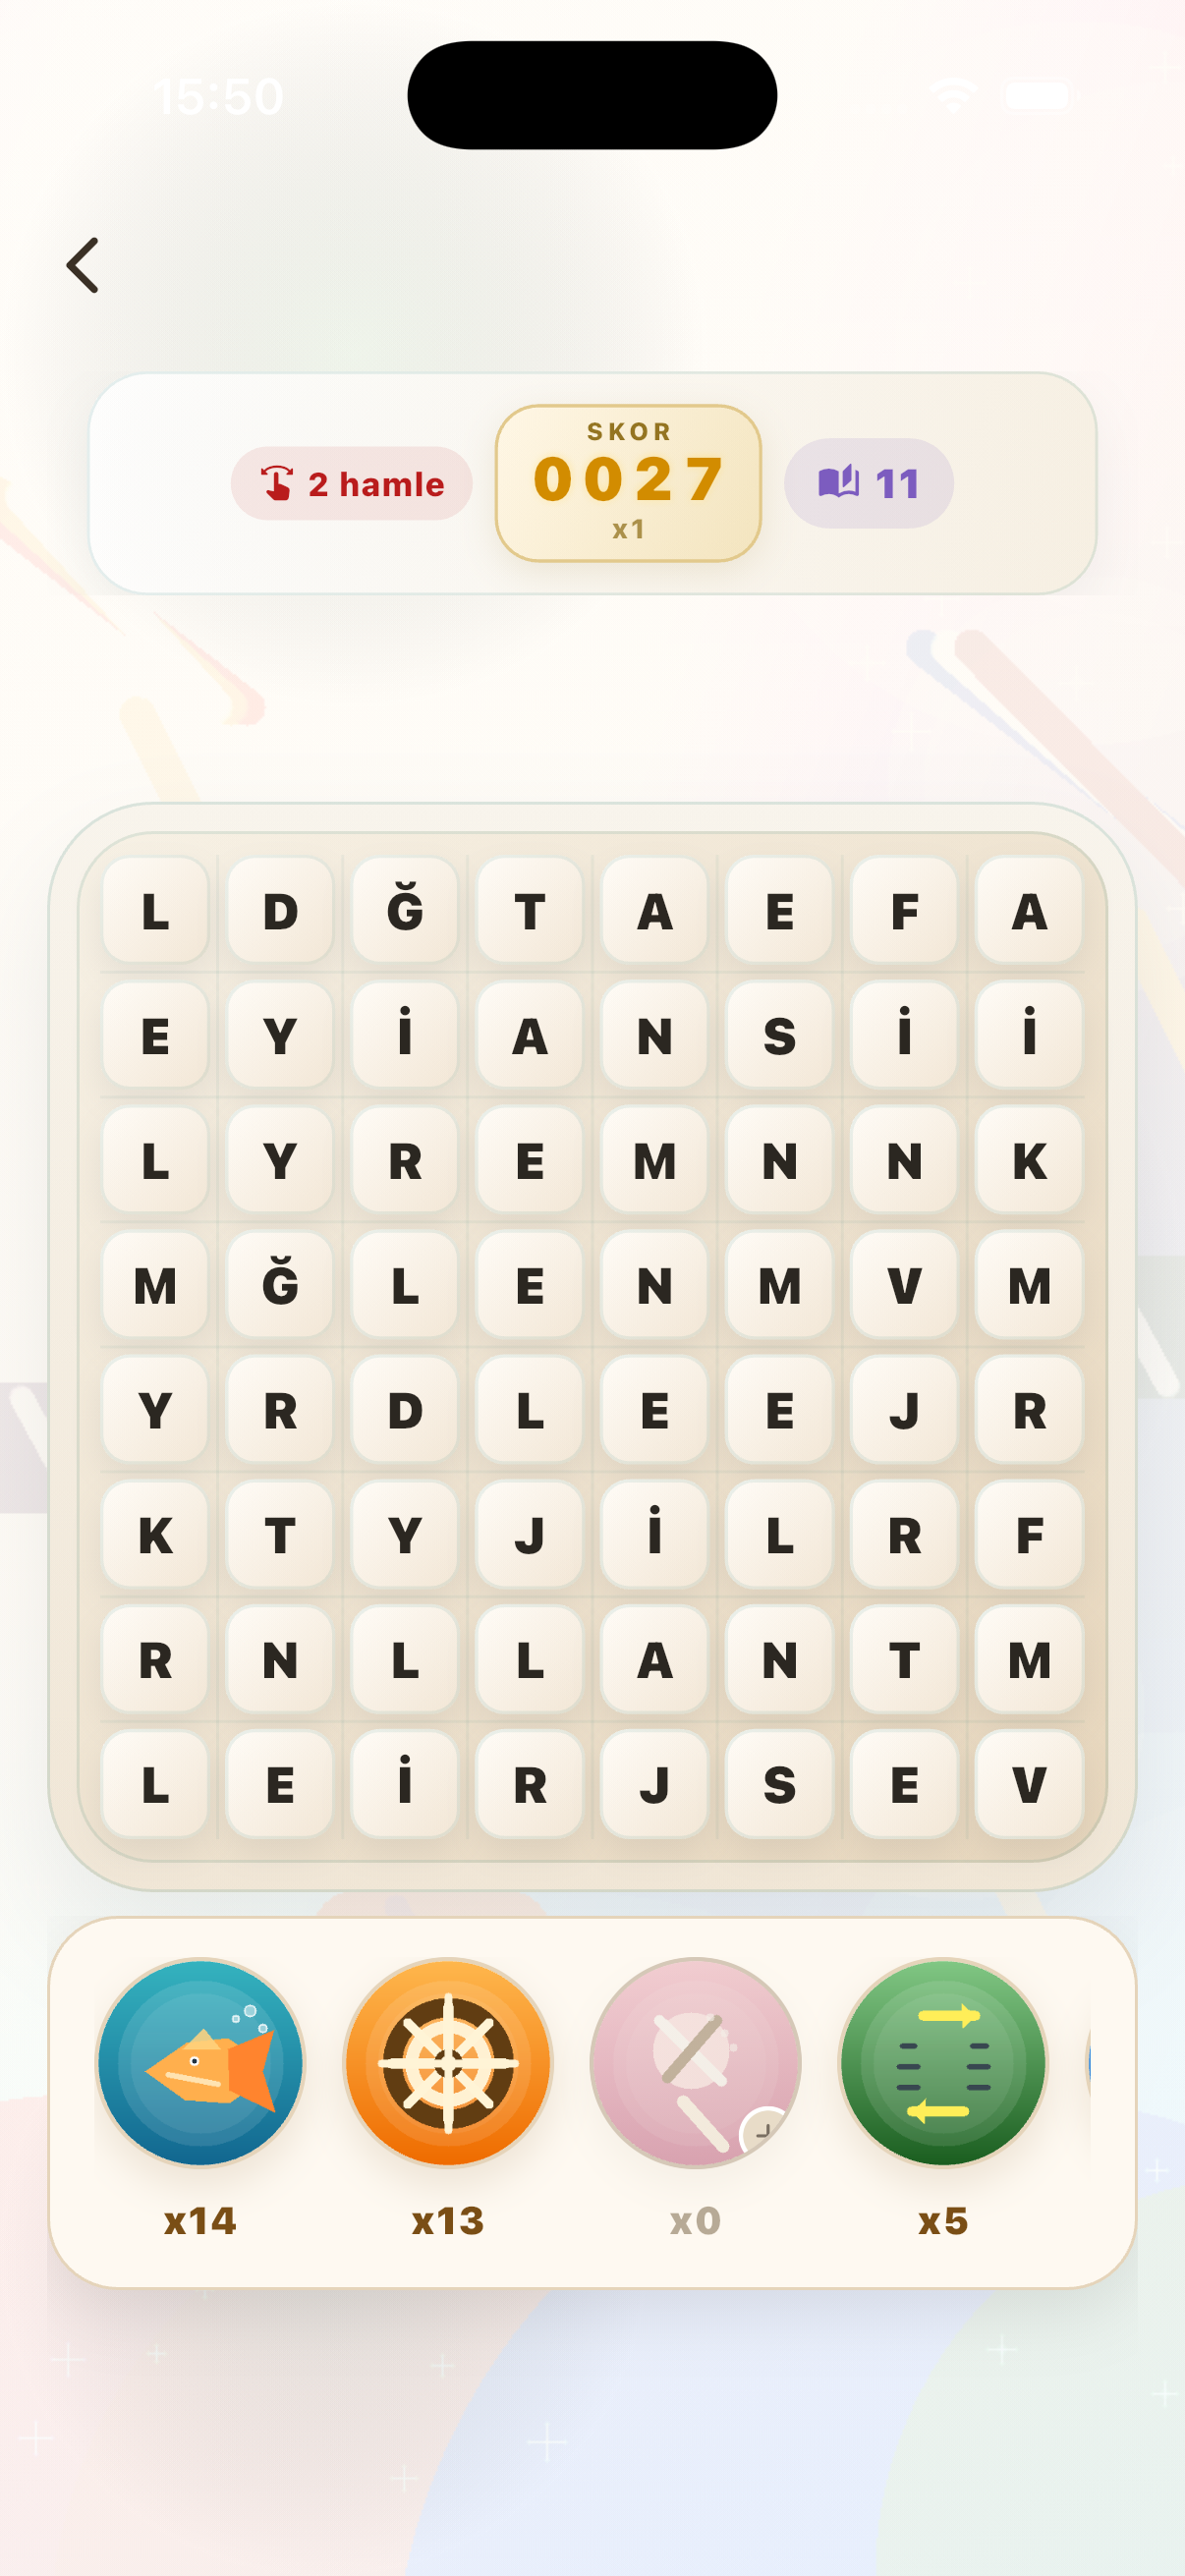
\includegraphics[width=0.57\linewidth]{game-board.png}}
  \caption{Oyun ekranı görünümü}
  \label{fig:game_screen}
\end{figure}

\subsection{Market Ekranı}

Market modülü, oyun içi joker ekonomisini yönetmektedir. Oyuncuya test amaçlı olarak başlangıçta yüksek miktarda oyun içi altın tanımlanmakta; gerçek para ile satın alma mekanizması bulunmamaktadır.

Market ekranında yer alan jokerler, işlevleri ve oyun içi maliyetleriyle birlikte Tablo~\ref{tab:market-jokers} üzerinde özetlenmiştir. Her jokerin açıklaması, maliyeti ve kullanım şekli detay ekranında sunulmaktadır.

Şekil~\ref{fig:market_screen} market ekranının görünümünü göstermektedir.

\begin{figure}[H]
  \centering
  \setlength{\fboxsep}{0pt}\fbox{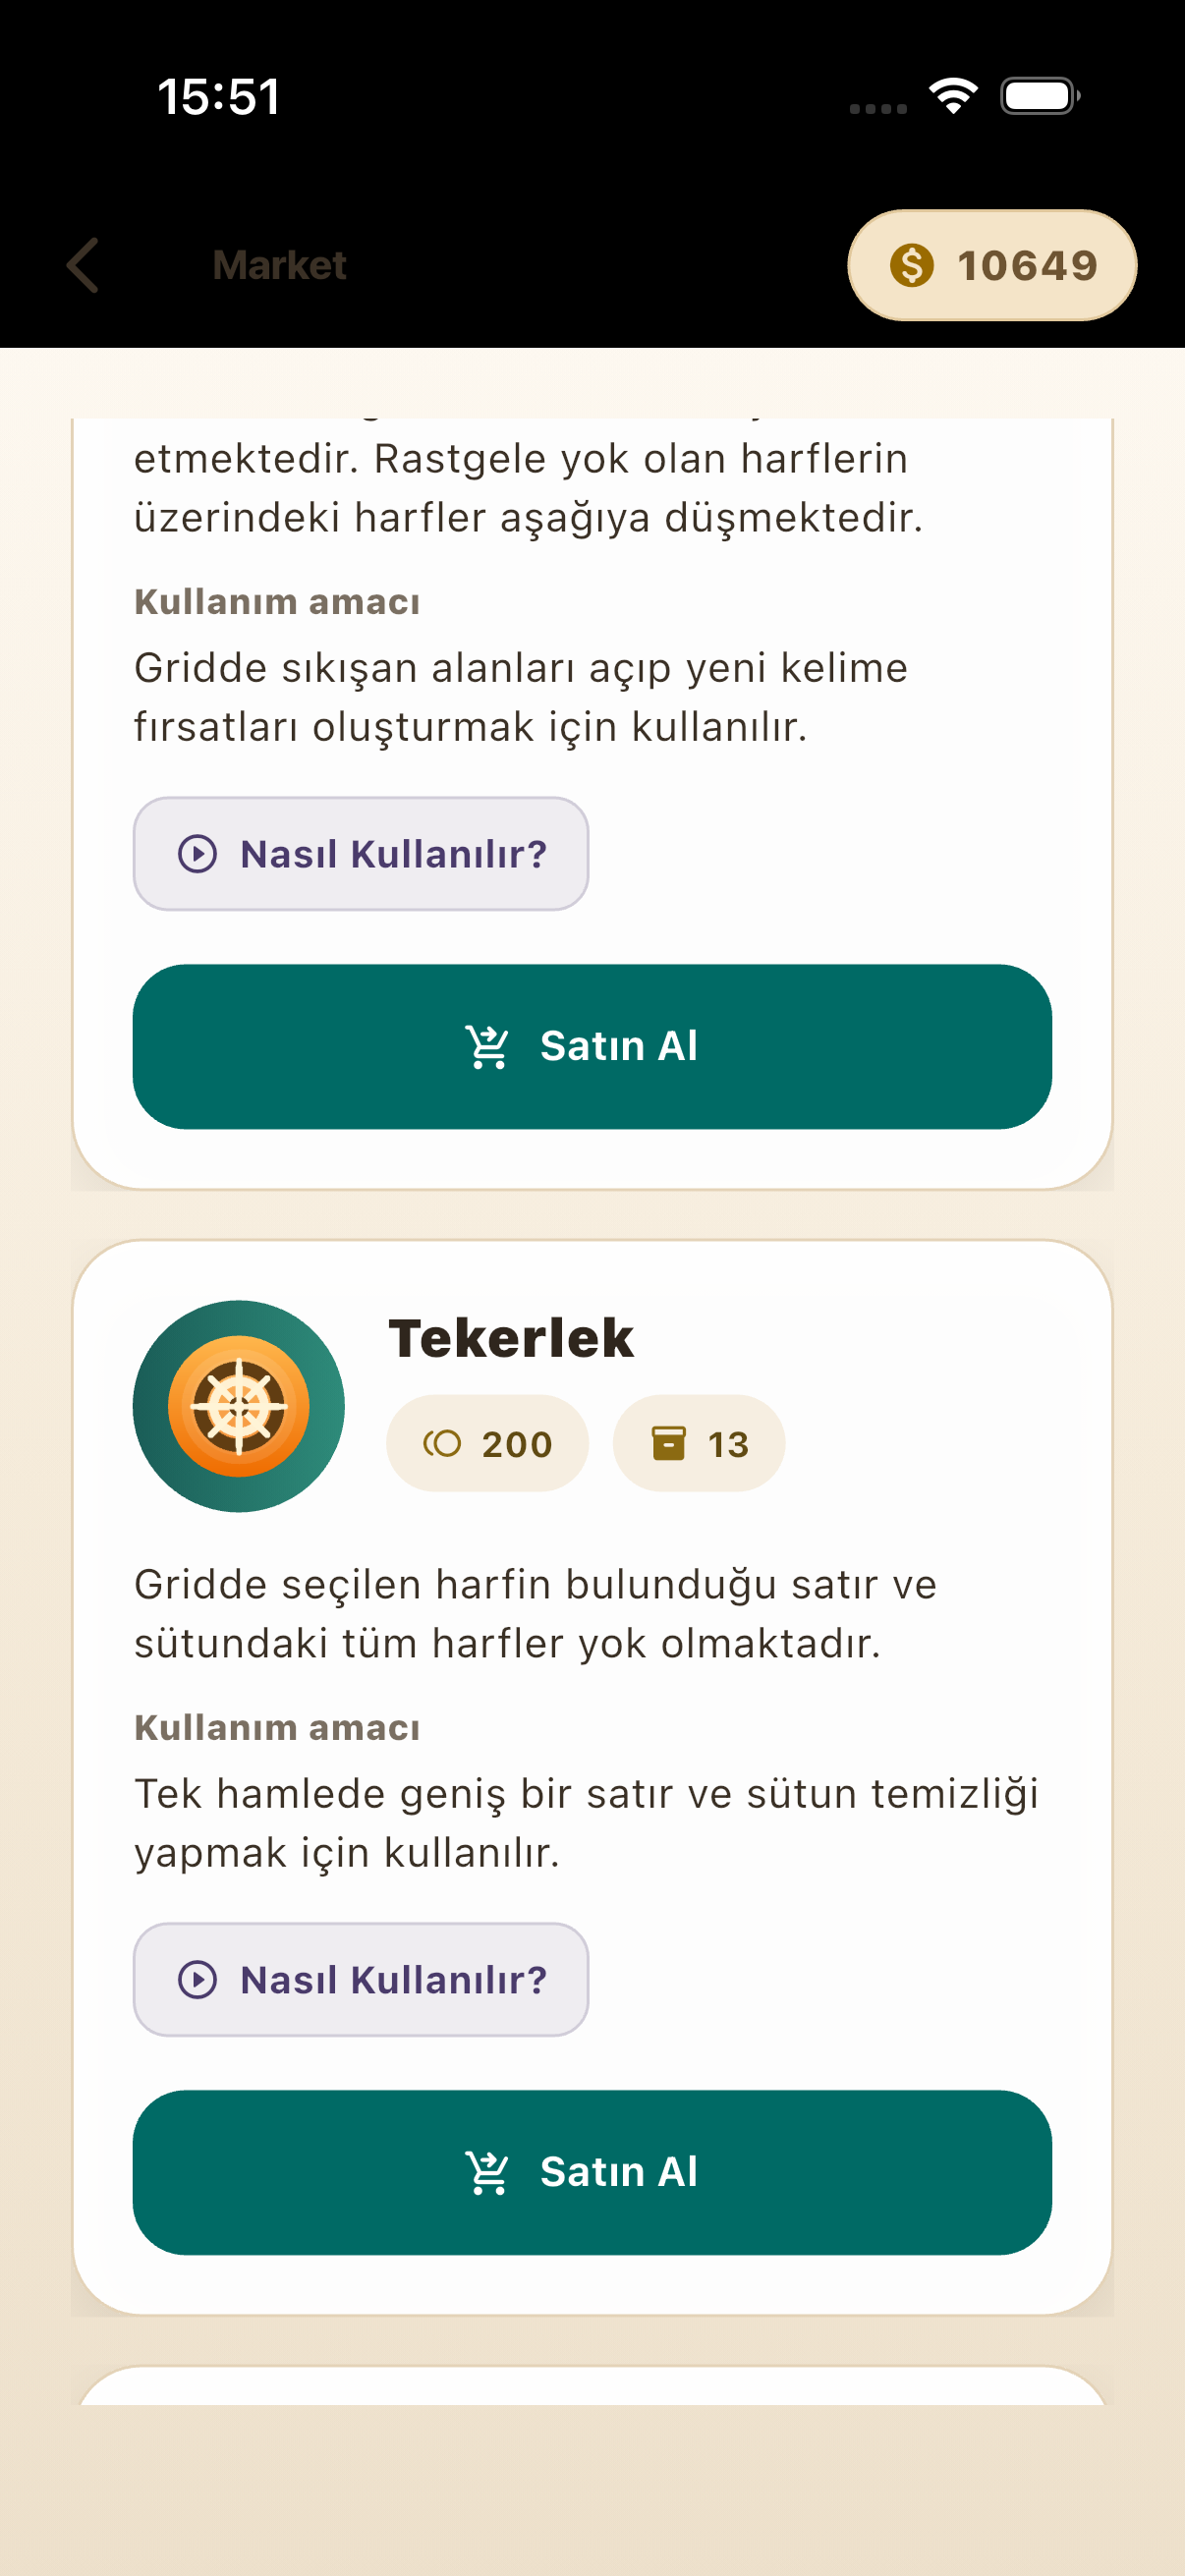
\includegraphics[width=0.57\linewidth]{market.png}}
  \caption{Market ekranı görünümü}
  \label{fig:market_screen}
\end{figure}

\begin{table}[!t]
\centering
\caption{Market ekranındaki jokerler ve maliyetleri}
\label{tab:market-jokers}
\begin{tabular}{lll}
\toprule
\textbf{Joker} & \textbf{İşlev} & \textbf{Maliyet} \\
\midrule
Balık & Rastgele harf yok eder & 100 altın \\
Tekerlek & Satır ve sütun temizler & 200 altın \\
Lolipop Kırıcı & Tek harf kaldırır & 75 altın \\
Serbest Değiştirme & Komşu iki harfin yerini değiştirir & 125 altın \\
Harf Karıştırma & Tüm tahtayı karıştırır & 300 altın \\
Parti Güçlendiricisi & Tahtayı tamamen sıfırlar & 400 altın \\
\bottomrule
\end{tabular}
\end{table}

\subsection{Skor Tablosu Ekranı}

Skor tablosu ekranı iki temel bölümden oluşmaktadır. Üst bölümde oyuncunun genel performansını özetleyen altı adet metrik yer almaktadır: toplam oynanan oyun sayısı, en yüksek puan, ortalama puan, toplam bulunan kelime sayısı, en uzun kelime ve toplam oyun süresi.

Alt bölümde tüm geçmiş oyunlar en son oynanan üste gelecek şekilde kronolojik sırada listelenmektedir. Her oyun kartında oyun numarası, tarih, grid boyutu, toplam puan, bulunan kelime sayısı, en uzun kelime ve oyun süresi bilgileri gösterilmektedir.

Şekil~\ref{fig:history_screen} skor tablosu ekranının görünümünü göstermektedir.

\begin{figure}[H]
  \centering
  \setlength{\fboxsep}{0pt}\fbox{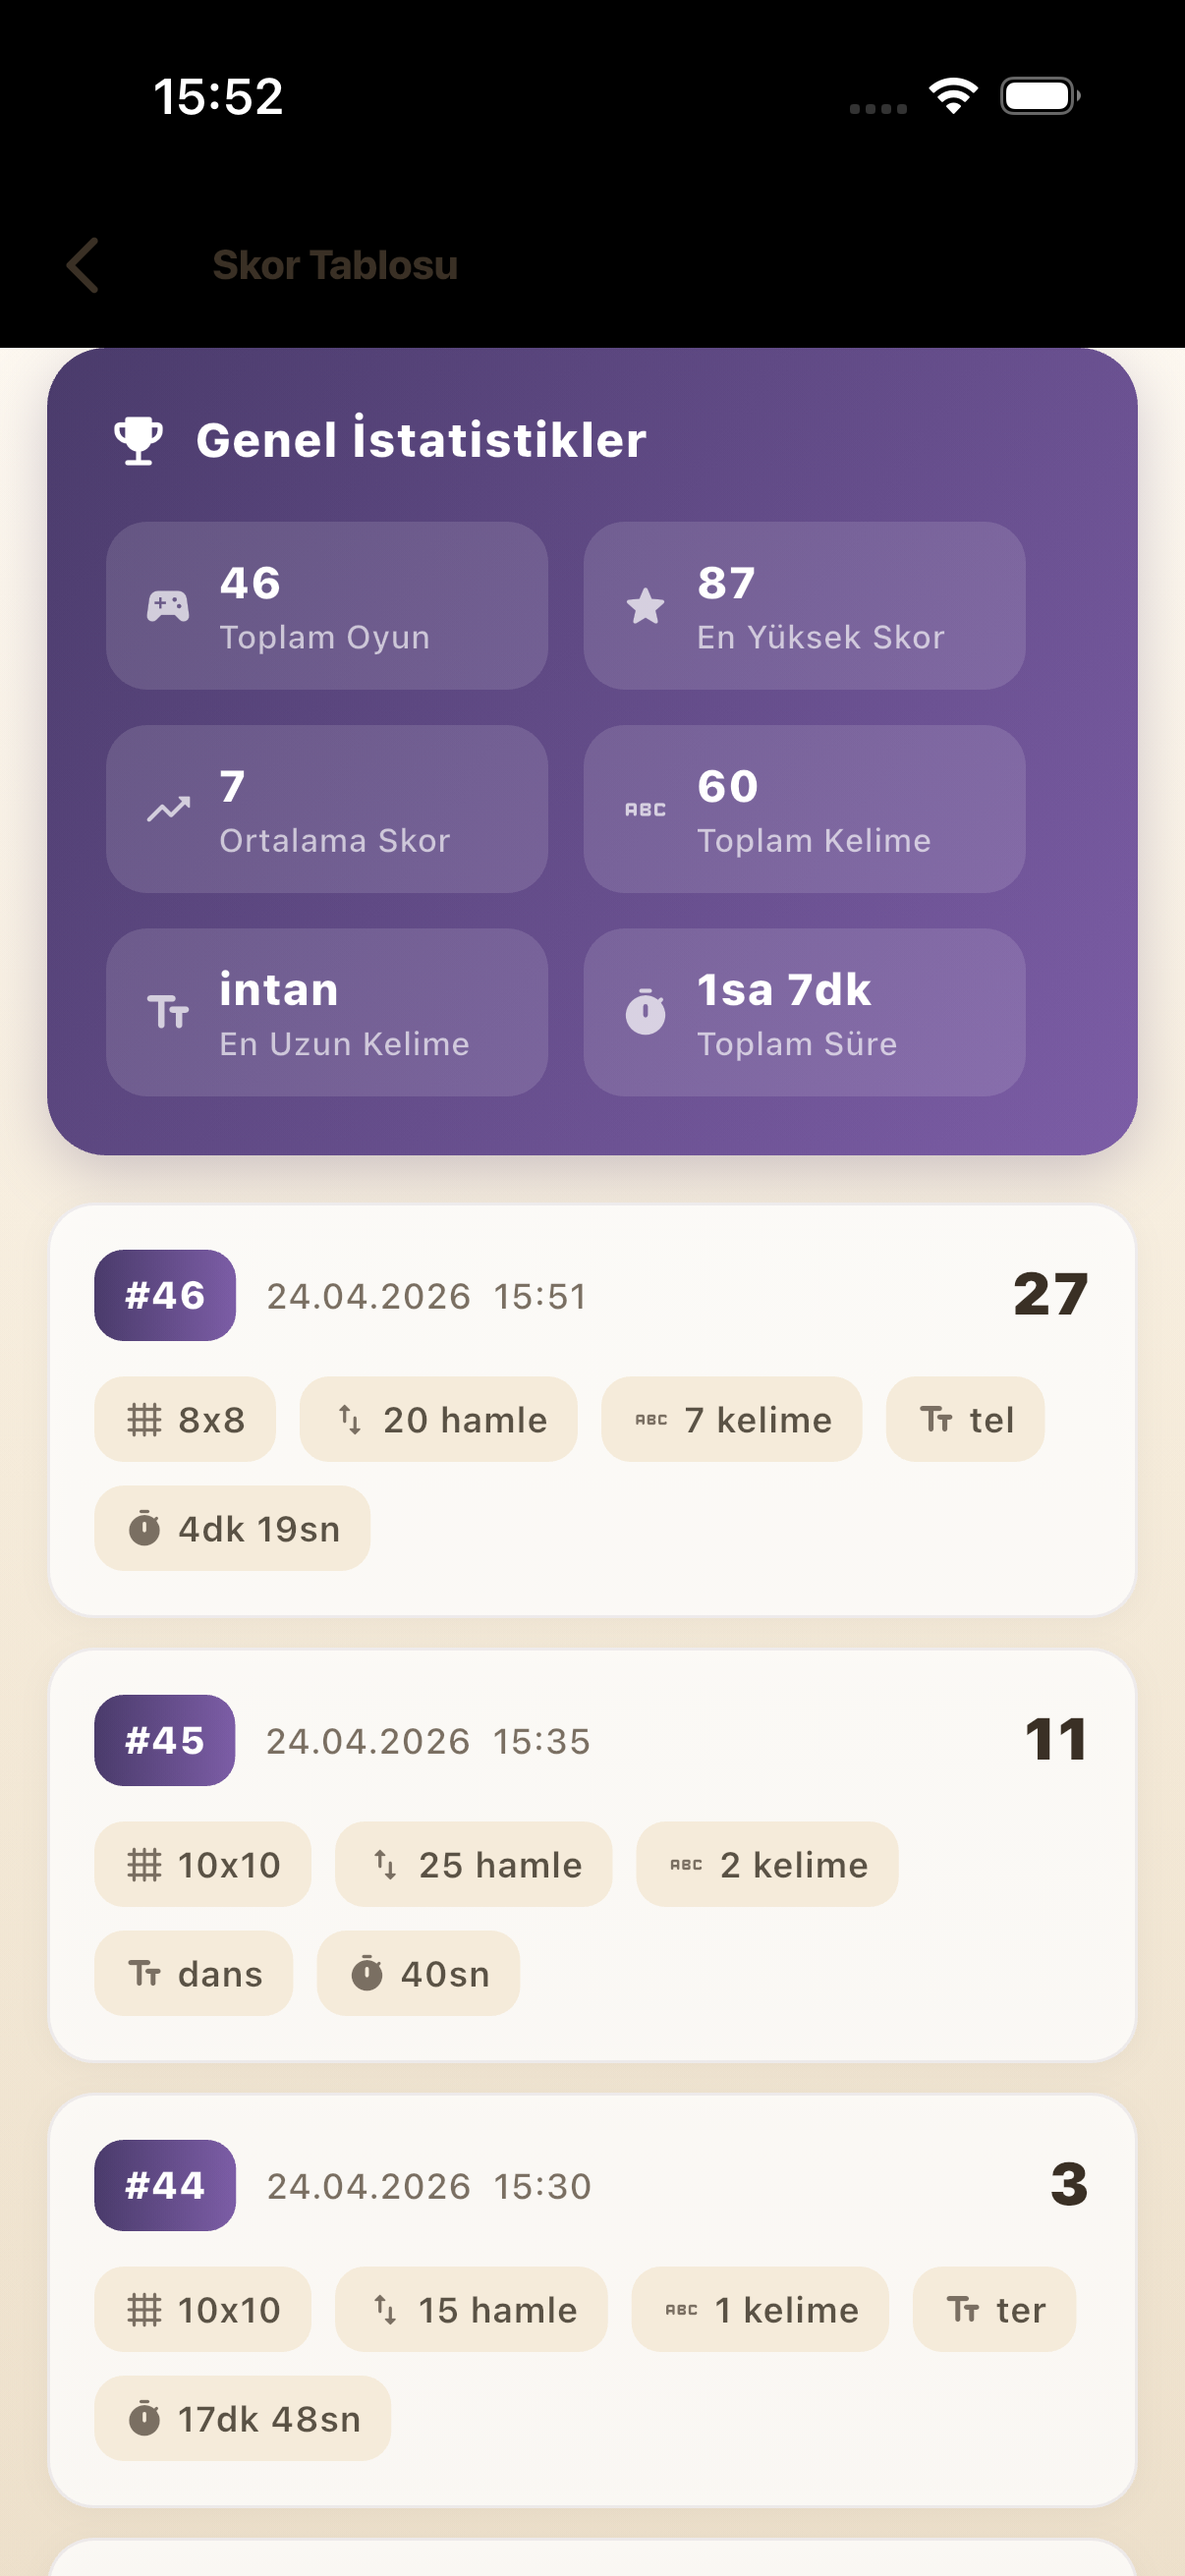
\includegraphics[width=0.57\linewidth]{scor-hist.png}}
  \caption{Skor tablosu ekranı görünümü}
  \label{fig:history_screen}
\end{figure}

% ================================================================
\section{Özel Güçler ve Combo Mekaniği}
% ================================================================

\subsection{Özel Güç Oluşturma}

Oyunda uzun kelimeler oluşturulması teşvik edilmektedir. Kelime uzunluğuna bağlı olarak son harfin bulunduğu konumda özel bir güç simgesi bırakılır. Bu simge daha sonra başka bir kelime içerisinde kullanıldığında ilgili güç aktif hale gelmektedir.

Özel güç türleri şu şekilde tanımlanmıştır: 4 harfli kelimeler satır temizleme gücü, 5 harfli kelimeler alan patlatma gücü, 6 harfli kelimeler sütun temizleme gücü ve 7 veya daha uzun kelimeler ise mega patlatma gücü oluşturmaktadır. Her özel gücün kendine özgü bir simgesi ve etki alanı bulunmaktadır.

\subsection{Combo Puanlama Mekanizması}

Combo mekanizması, oyuncunun oluşturduğu ana kelimenin içerisinde yer alan anlamlı bitişik alt kelimelerin de ek puan kazandırmasını sağlayan bir yapıdır. Alt kelime tespitinde aşağıdaki kurallar uygulanır:

\begin{itemize}
  \item Alt kelime en az 3 harf uzunluğunda olmalıdır.
  \item Alt kelimeler ana kelimenin harf sırasını koruyan bitişik parçalar olmalıdır.
  \item Aynı alt kelime birden fazla kez sayılamaz.
  \item Ana kelime her zaman combo sayısına dahildir.
\end{itemize}

Örneğin ``YAZAR'' kelimesi içinde YAZ ve AZAR alt kelimeleri tespit edildiğinde, ana kelimeyle birlikte toplam 3 combo oluşur ve ilgili kelimelerin puanları birlikte hesaplanır.

% ================================================================
\section{Oyun Sonu ve Sonuç Kaydı}
% ================================================================

Oyun iki farklı durumda sona ermektedir. Birinci durumda oyuncunun hamle sayısı sıfırlandığında oyun otomatik olarak biter ve mevcut sonuç yerel veritabanına kaydedilir. İkinci durumda oyuncu geri tuşuna basarak oyundan çıkmak istediğinde ``Çıkmak istediğinize emin misiniz?'' onay diyaloğu gösterilir. ``Evet'' seçiminde mevcut oyun sonucu kaydedilip aktif oturum temizlenerek ana ekrana dönülür; ``Hayır'' seçiminde ise oyun kesintisiz biçimde sürdürülür. Ayrıca aktif oyun oturumu, oyun devam ederken yerel kontrol noktası mantığıyla saklanarak akışın güvenilirliği artırılmaktadır.

Kaydedilen oyun sonucu; tamamlanma zamanı, zorluk seviyesi, tahta boyutu, başlangıç hamle sayısı, elde edilen puan, bulunan kelime sayısı, en uzun kelime ve toplam oyun süresini içerir. Bu veriler skor tablosu ekranında kullanıcıya sunulmaktadır.

% ================================================================
\section{Test ve Değerlendirme}
% ================================================================

Proje kapsamında birim test ve bileşen testi yaklaşımı uygulanmıştır. Yerçekimi ve yeniden doldurma işlemlerinin doğruluğu, puanlama hesaplarının tutarlılığı, kelime doğrulama mekanizmasının davranışı, tahta çözülebilirlik analizinin sonuçları, kurtarma stratejilerinin beklenen çıktıları, combo puanlama, özel güç oluşturma ve etkinleştirme kuralları ile aktif oturumun yerel olarak saklanması birim testler ile doğrulanmıştır.

Kullanıcı arayüzü katmanında ise kullanıcı adı alma akışı, yeni oyun kurulumu, oyun ekranındaki seçim davranışı, joker çubuğu, market ekranı, oyun sonu akışı ve skor tablosu ekranının doğru bilgileri gösterdiği bileşen testleri ile teyit edilmiştir. Statik kod analiz araçlarıyla kod kalite kontrolleri başarıyla geçmiştir.

Testler aşağıdaki alanları kapsamaktadır:

\begin{itemize}
  \item Tahta çözülebilirlik analiz algoritması (Trie oluşturma, DFS gezinme, prefix budama)
  \item Tahta kurtarma stratejisi (karıştırma ve yeniden üretim adımları)
  \item Kelime doğrulama (minimum uzunluk, sözlük kontrolü)
  \item Puanlama hesabı (harf bazlı puan toplamı)
  \item Combo puanlama ve alt kelime tespiti
  \item Kelime uzunluğuna bağlı özel güç oluşturma ve etki uygulama kuralları
  \item Yerçekimi ve yeniden doldurma çözümlemesi
  \item Aktif oyun oturumu saklama ve temizleme akışı
  \item Hamle sonrası oynanabilir tahta koruma ve oluşturulabilir kelime sayısı güncelleme mantığı
  \item Oyun sonu ve sonuç kaydetme akışı
  \item Kullanıcı adı giriş akışı ve yeni oyun kurulum ekranları
  \item Market ekranı, joker satın alma ve oyun içi joker erişimi
  \item Skor tablosu özet metrikleri ve liste görünümü
\end{itemize}

% ================================================================
\section{Sonuç}
% ================================================================

Bu çalışmada, mobil platformlar için Türkçe kelime bulma tabanlı bir oyun başarıyla geliştirilmiştir. Uygulama; ağırlıklı harf üretim algoritması, Trie tabanlı tahta analiz mekanizması, yerçekimi ve yeniden doldurma mekaniği, combo puanlama, özel güç üretimi, SQLite ile yerel kalıcı veri yönetimi, aktif oturum saklama ve market ekonomisi gibi temel bileşenlerden oluşmaktadır.

Projenin mevcut tamamlanma durumu şu şekilde özetlenebilir: platform ve kapsam, kullanıcı yönetimi, ana ekran, oyun kurulumu, temel grid ve kelime kuralları, puanlama sistemi, combo mekanikleri, özel güç üretimi ve tetikleme mantığı, joker satın alma ve kullanım akışı, aktif oturum yönetimi ile oyun sonu akışları başarıyla uygulanmıştır. Böylece proje yalnızca temel kelime bulma deneyimini değil, aynı zamanda süreklilik ve çeşitlilik sağlayan yardımcı oyun mekaniklerini de içeren bütüncül bir yapıya ulaşmıştır.

% ================================================================

\bibliographystyle{IEEEtran}
\bibliography{references}

\end{document}
